
\section{result}

\begin{figure}[!h]
    \centering
    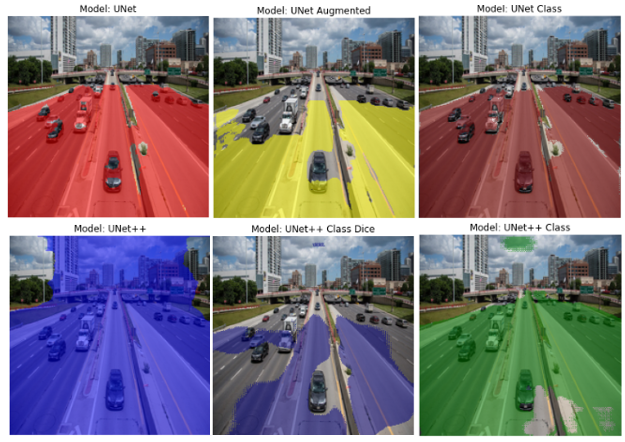
\includegraphics[width=1\linewidth]{dron_view.png} % 그림 파일 이름과 너비 설정
    \caption{드론 카메라 위치에서 촬영된 사진에 대한 모델 비교 결과} % 캡션 추가
    \label{fig:road_detection} % 레이블 설정 (참조용)
\end{figure}

자율주행 데이터에서 도로 결함을 검출하는 각 모델의 성능을 평가하고, 저공 비행 드론에 적용했을 때의 성능 변화를 분석한다. 실험 결과는 다음과 같다.
\begin{figure}[!h]
    \centering
    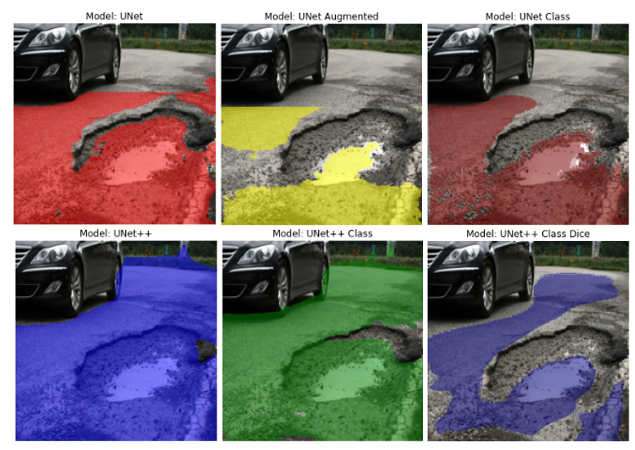
\includegraphics[width=1\linewidth]{lane_crack.png} % 그림 파일 이름과 너비 설정
    \caption{도로 결함에 대한 각 모델 비교 결과} % 캡션 추가
    \label{fig:crack_detection} % 레이블 설정 (참조용)
\end{figure}

\subsection{이진 분류 세그멘테이션 결과}
U-Net 모델은 구조가 단순하여 연산 속도가 빠르고, 다양한 조명 조건에서도 안정적인 성능을 보였다. U-Net++ 모델은 Dice 손실을 사용하여 불균형 데이터 상황에서 더욱 우수한 결함 탐지 성능을 나타냈다.

\subsection{다중 클래스 세그멘테이션 결과}
다중 클래스 세그멘테이션에서는 U-Net++ 모델이 U-Net 모델보다 높은 성능을 보였다. 특히 Dice 손실을 추가하여 불균형 클래스에 대한 성능이 개선되었으며, Road IoU 메트릭을 통해 세분화된 결함 탐지 성능이 측정되었다.

\subsection{손실 함수와 메트릭의 영향}
Dice 손실을 적용한 U-Net++ 모델에서는 다중 클래스 세그멘테이션 성능이 유의미하게 향상되었으며, Dice 계수와 Road IoU를 동시에 사용하는 것이 정확도를 높이는 데 기여하였다.

